\chapter{Diseño de la persistencia de la información}
\label{cap:persistenciaInformacion}

Este capítulo presenta el diseño físico de almacenamiento de la información de \textbf{Taimotla}. Se incluye la representación del Modelo Relacional de base de datos, el Diccionario de datos para las entidades críticas del sistema y el Diccionario de consultas lógicas parametrizadas ejecutadas por el backend.

%---------------------------------------------------------
\section{Modelo Relacional}
\label{sec:modeloRelacional}

La base de datos relacional de \textbf{Taimotla} está construida en PostgreSQL. Su estructura consta de 45 tablas normalizadas para evitar redundancias y asegurar integridad. En la figura~\ref{fig:modeloRelacionalDB} se presenta el diagrama del Modelo Relacional físico del sistema.

\begin{figure}[htbp!]
\centering
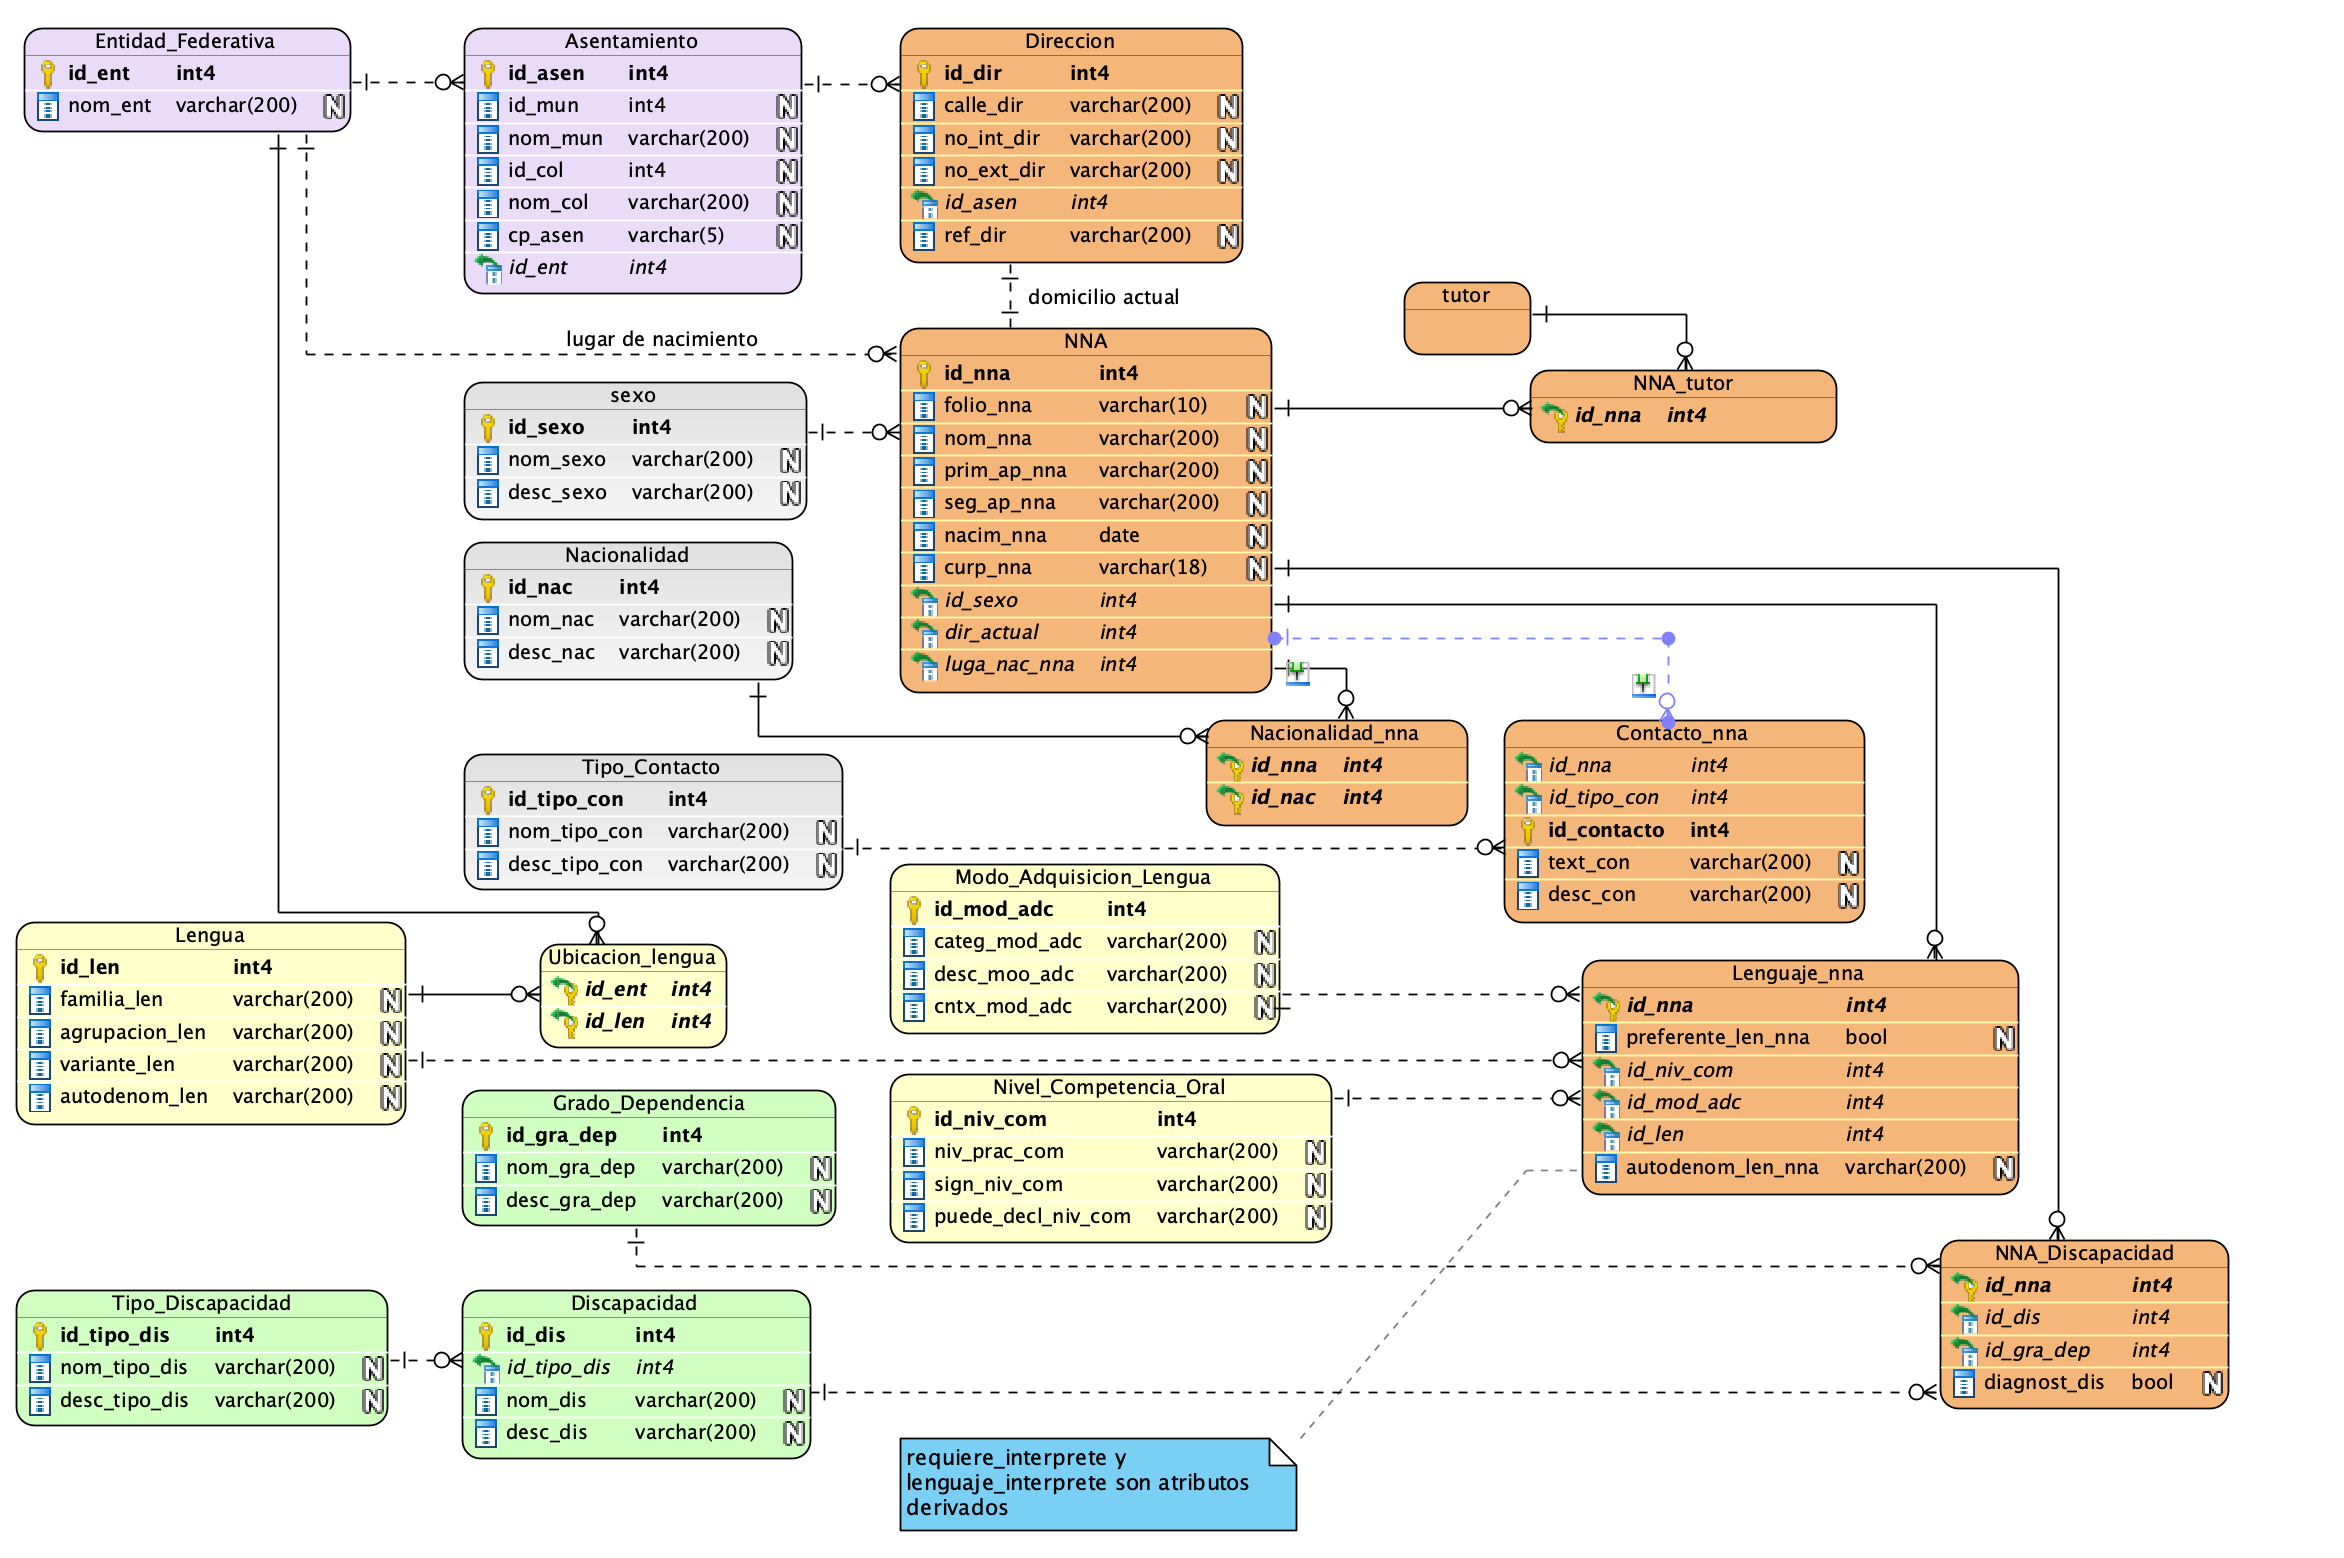
\includegraphics[width=0.95\textwidth]{images/modelo_relacional}
\caption{Diagrama del Modelo Relacional Físico de la Base de Datos.}
\label{fig:modeloRelacionalDB}
\end{figure}

%---------------------------------------------------------
\section{Diccionario de datos}
\label{sec:diccionarioDatos}

A continuación se describen las especificaciones de almacenamiento e integridad para las tablas fundamentales del sistema:

\subsection{Tabla: persona}
Almacena la identidad general de toda persona registrada en el sistema (empleados, tutores o menores).
\begin{table}[htbp!]
\centering
\begin{tabular}{|l|l|l|c|l|}
\hline
\textbf{Columna} & \textbf{Tipo de Dato} & \textbf{Llave} & \textbf{Null} & \textbf{Descripción / Restricción} \\
\hline
CURP & character varying(18) & PK & No & Clave única de población. Identificador. \\
RFC & character varying(13) & Unique & No & Registro Federal de Contribuyentes. \\
p\_nombre & character varying(50) & - & No & Primer nombre. \\
s\_nombre & character varying(50) & - & Sí & Segundo nombre (opcional). \\
p\_apellido & character varying(50) & - & No & Primer apellido. \\
s\_apellido & character varying(50) & - & No & Segundo apellido. \\
fecha\_nacimiento & date & - & No & Fecha de nacimiento. \\
id\_sexo\_persona & integer & FK & Sí & Sexo biológico (ref. tabla \texttt{sexo}). \\
id\_domicilio\_persona & integer & FK & Sí & Domicilio (ref. tabla \texttt{domicilio}). \\
id\_correo & integer & FK & Sí & Correo electrónico (ref. tabla \texttt{correos}). \\
\hline
\end{tabular}
\caption{Diccionario de datos de la tabla \texttt{persona}.}
\label{tbl:diccionarioPersona}
\end{table}

\subsection{Tabla: personal}
Registra los accesos y estatus de los empleados de la Fundación.
\begin{table}[htbp!]
\centering
\begin{tabular}{|l|l|l|c|l|}
\hline
\textbf{Columna} & \textbf{Tipo de Dato} & \textbf{Llave} & \textbf{Null} & \textbf{Descripción / Restricción} \\
\hline
CURP & character varying(18) & PK, FK & No & CURP del empleado (ref. tabla \texttt{persona}). \\
fecha\_alta & date & - & No & Fecha de ingreso. \\
voluntario & boolean & - & No & Indica si es personal voluntario. \\
contrasena & character varying(255) & - & No & Contraseña cifrada con hash. \\
estado & integer & FK & Sí & Estatus de cuenta (ref. tabla \texttt{estado\_cuenta}). \\
\hline
\end{tabular}
\caption{Diccionario de datos de la tabla \texttt{personal}.}
\label{tbl:diccionarioPersonal}
\end{table}

\subsection{Tabla: nna}
Registra los menores sujetos a medidas de restitución de derechos.
\begin{table}[htbp!]
\centering
\begin{tabular}{|l|l|l|c|l|}
\hline
\textbf{Columna} & \textbf{Tipo de Dato} & \textbf{Llave} & \textbf{Null} & \textbf{Descripción / Restricción} \\
\hline
id\_nna & serial & PK & No & Clave autoincremental única. \\
id\_persona\_exp\_nna & integer & FK & No & Datos personales del menor (ref. \texttt{personas\_expediente}). \\
id\_expediente & integer & FK & Sí & Expediente asociado (ref. tabla \texttt{expediente}). \\
apodo & character varying(50) & - & Sí & Apodo o nombre de confianza. \\
observaciones & character varying(100) & - & Sí & Notas generales sobre el menor. \\
id\_etnia & integer & FK & Sí & Etnia de origen (ref. tabla \texttt{etnia}). \\
id\_nacionalidad & integer & FK & Sí & Nacionalidad (ref. tabla \texttt{nacionalidad}). \\
\hline
\end{tabular}
\caption{Diccionario de datos de la tabla \texttt{nna}.}
\label{tbl:diccionarioNna}
\end{table}

\subsection{Tabla: equipo}
Almacena la información de identificación y estado de los grupos multidisciplinarios creados.
\begin{table}[htbp!]
\centering
\begin{tabular}{|l|l|l|c|l|}
\hline
\textbf{Columna} & \textbf{Tipo de Dato} & \textbf{Llave} & \textbf{Null} & \textbf{Descripción / Restricción} \\
\hline
id\_equipo & serial & PK & No & Identificador autoincremental del equipo. \\
nombre\_equipo & character varying(50) & - & Sí & Nombre distintivo del equipo. \\
fecha\_creacion & date & - & No & Fecha de creación del equipo. \\
curp\_coordinador & character varying(18) & FK & No & CURP del coordinador (ref. \texttt{coordinador}). \\
id\_estado\_equipo & integer & FK & Sí & Estado de activación (ref. \texttt{estado\_equipo}). \\
\hline
\end{tabular}
\caption{Diccionario de datos de la tabla \texttt{equipo}.}
\label{tbl:diccionarioEquipo}
\end{table}

\subsection{Tabla: composicion\_equipo}
Registra el historial de asignaciones de profesionales especialistas a cada equipo.
\begin{table}[htbp!]
\centering
\begin{tabular}{|l|l|l|c|l|}
\hline
\textbf{Columna} & \textbf{Tipo de Dato} & \textbf{Llave} & \textbf{Null} & \textbf{Descripción / Restricción} \\
\hline
id\_asignacion & serial & PK & No & Identificador único de la asignación. \\
id\_equipo & integer & FK & No & Identificador del equipo (ref. \texttt{equipo}). \\
curp\_profesional & character varying(18) & FK & No & CURP del especialista (ref. \texttt{personal}). \\
fecha\_inicio & date & - & No & Fecha de incorporación al equipo. \\
fecha\_fin & date & - & Sí & Fecha de salida o término en el equipo. \\
\hline
\end{tabular}
\caption{Diccionario de datos de la tabla \texttt{composicion\_equipo}.}
\label{tbl:diccionarioComposicion}
\end{table}

\subsection{Tabla: expediente}
Almacena los datos generales del expediente de seguimiento del menor.
\begin{table}[htbp!]
\centering
\begin{tabular}{|l|l|l|c|l|}
\hline
\textbf{Columna} & \textbf{Tipo de Dato} & \textbf{Llave} & \textbf{Null} & \textbf{Descripción / Restricción} \\
\hline
id\_expediente & serial & PK & No & Identificador único interno del expediente. \\
num\_expediente & character varying(20) & Unique & No & Número o folio oficial del expediente. \\
fecha\_apertura & timestamp & - & No & Fecha y hora de creación. \\
id\_equipo\_responsable & integer & FK & Sí & Equipo asignado al seguimiento (ref. \texttt{equipo}). \\
id\_estado\_expediente & integer & FK & Sí & Estado del expediente (ref. \texttt{estado\_expediente}). \\
\hline
\end{tabular}
\caption{Diccionario de datos de la tabla \texttt{expediente}.}
\label{tbl:diccionarioExpediente}
\end{table}

\subsection{Tabla: tutores}
Registra la información sociofamiliar y laboral de los tutores o cuidadores de los menores.
\begin{table}[htbp!]
\centering
\begin{tabular}{|l|l|l|c|l|}
\hline
\textbf{Columna} & \textbf{Tipo de Dato} & \textbf{Llave} & \textbf{Null} & \textbf{Descripción / Restricción} \\
\hline
id\_tutor & serial & PK & No & Identificador único del tutor. \\
id\_persona\_exp & integer & FK & No & Referencia a datos personales (ref. \texttt{personas\_expediente}). \\
ocupacion & character varying(50) & - & No & Actividad laboral u ocupación principal. \\
es\_sosten\_economico & boolean & - & No & Indica si es el principal sostén económico del hogar. \\
observaciones & character varying(100) & - & Sí & Comentarios adicionales del Trabajador Social. \\
escolaridad & character varying(50) & - & No & Grado escolar máximo alcanzado. \\
patron\_migracion & character varying(100) & - & Sí & Descripción de flujos de movilidad familiar. \\
id\_telefono & integer & FK & Sí & Teléfono de contacto (ref. \texttt{telefonos\_tutores}). \\
id\_correo & integer & FK & Sí & Correo de contacto (ref. \texttt{correos\_tutores}). \\
id\_parentesco & integer & FK & Sí & Relación con el menor (ref. \texttt{parentesco}). \\
id\_grado\_negacion & integer & FK & Sí & Grado de negación del hecho (ref. \texttt{grado\_negacion}). \\
id\_grado\_afectacion\_emocional & integer & FK & Sí & Nivel de afectación (ref. \texttt{grado\_afectacion\_emocional}). \\
\hline
\end{tabular}
\caption{Diccionario de datos de la tabla \texttt{tutores}.}
\label{tbl:diccionarioTutores}
\end{table}

\subsection{Tabla: familiares}
Registra los demás integrantes de la red familiar o de apoyo del menor en el expediente.
\begin{table}[htbp!]
\centering
\begin{tabular}{|l|l|l|c|l|}
\hline
\textbf{Columna} & \textbf{Tipo de Dato} & \textbf{Llave} & \textbf{Null} & \textbf{Descripción / Restricción} \\
\hline
id\_familiar & serial & PK & No & Identificador único del familiar. \\
id\_persona\_exp & integer & FK & No & Datos personales del familiar (ref. \texttt{personas\_expediente}). \\
parentesco & character varying(50) & - & No & Tipo de parentesco con el menor. \\
observaciones & character varying(100) & - & Sí & Notas o datos relevantes de la red de apoyo. \\
\hline
\end{tabular}
\caption{Diccionario de datos de la tabla \texttt{familiares}.}
\label{tbl:diccionarioFamiliares}
\end{table}

\subsection{Tabla: hecho\_victimal}
Almacena el reporte detallado del suceso de detención o vulneración que motivó el expediente.
\begin{table}[htbp!]
\centering
\begin{tabular}{|l|l|l|c|l|}
\hline
\textbf{Columna} & \textbf{Tipo de Dato} & \textbf{Llave} & \textbf{Null} & \textbf{Descripción / Restricción} \\
\hline
id\_hecho & serial & PK & No & Identificador único del hecho victimal. \\
id\_nna & integer & FK & Sí & Identificador del menor asociado (ref. \texttt{nna}). \\
num\_reporte & character varying(100) & - & No & Folio del reporte de detención u origen. \\
nombre\_caso & character varying(100) & - & No & Nombre identificativo asignado al caso. \\
fecha\_detencion & date & - & No & Fecha en que ocurrió el suceso. \\
nombre\_victima\_madre & character varying(100) & - & No & Nombre de la madre de la víctima. \\
descripcion\_delito & character varying(100) & - & Sí & Delitos presuntos identificados. \\
narracion\_sucedido & character varying(100) & - & Sí & Breve síntesis del relato del suceso. \\
id\_tipo\_detector & integer & FK & Sí & Quien detectó la situación (ref. \texttt{tipo\_detector}). \\
id\_direccion\_delito & integer & FK & Sí & Dirección del lugar (ref. \texttt{domicilio\_servicios}). \\
\hline
\end{tabular}
\caption{Diccionario de datos de la tabla \texttt{hecho\_victimal}.}
\label{tbl:diccionarioHecho}
\end{table}

%---------------------------------------------------------
\section{Diseño de las consultas}
\label{sec:disenoConsultas}

Las consultas ejecutadas en el backend se diseñan de forma parametrizada para evitar inyecciones de código SQL y asegurar un óptimo rendimiento en el servidor PostgreSQL. A continuación se expone el diccionario de consultas detallado:

\subsection{Diccionario de consultas}

\subsubsection{Consulta: Query1 (Verificar Director)}
\begin{description}
    \item[Nombre:] Query1
    \item[Parámetros:] email: string
    \item[Diseño:] \cdtEmpty
\end{description}
\begin{verbatim}
SELECT p."CURP",
       p.p_nombre,
       pers.contrasena,
       pers.estado
FROM   public.correos      c
JOIN   public.persona      p    ON c.id_correo = p.id_correo
JOIN   public.personal     pers ON p."CURP"    = pers."CURP"
JOIN   public.director     d    ON p."CURP"    = d."CURP"
WHERE  c.correo = %s;
\end{verbatim}

\subsubsection{Consulta: Query2 (Verificar Coordinador)}
\begin{description}
    \item[Nombre:] Query2
    \item[Parámetros:] email: string
    \item[Diseño:] \cdtEmpty
\end{description}
\begin{verbatim}
SELECT p."CURP",
       p.p_nombre,
       pers.contrasena,
       pers.estado
FROM   public.correos      c
JOIN   public.persona      p    ON c.id_correo = p.id_correo
JOIN   public.personal     pers ON p."CURP"    = pers."CURP"
JOIN   public.coordinador  co   ON p."CURP"    = co."CURP"
WHERE  c.correo = %s;
\end{verbatim}

\subsubsection{Consulta: Query3 (Consultar Expediente del NNA)}
\begin{description}
    \item[Nombre:] Query3
    \item[Parámetros:] num\_expediente: string
    \item[Diseño:] \cdtEmpty
\end{description}
\begin{verbatim}
SELECT n.id_nna,
       pe.p_nombre,
       pe.p_apellido,
       e.num_expediente,
       e.id_expediente,
       e.id_estado_expediente
FROM   public.nna                 n
JOIN   public.personas_expediente pe ON n.id_persona_exp_nna = pe.id_persona_exp
JOIN   public.expediente          e  ON n.id_expediente      = e.id_expediente
WHERE  e.num_expediente = %s;
\end{verbatim}

\subsubsection{Consulta: Query4 (Creación de Equipos)}
\begin{description}
    \item[Nombre:] Query4
    \item[Parámetros:] nombre\_equipo: string, curp\_coordinador: string, id\_estado\_equipo: int
    \item[Diseño:] \cdtEmpty
\end{description}
\begin{verbatim}
INSERT INTO public.equipo (nombre_equipo, curp_coordinador, id_estado_equipo)
VALUES (%s, %s, %s);
\end{verbatim}

\subsubsection{Consulta: Query5 (Obtener todos los Especialistas de un Equipo)}
\begin{description}
    \item[Nombre:] Query5
    \item[Parámetros:] id\_equipo: int
    \item[Diseño:] \cdtEmpty
\end{description}
\begin{verbatim}
SELECT p."CURP",
       pe.p_nombre,
       pe.p_apellido,
       pers.voluntario
FROM   public.composicion_equipo ce
JOIN   public.personal           pers ON ce.curp_profesional = pers."CURP"
JOIN   public.persona            pe   ON pers."CURP"         = pe."CURP"
WHERE  ce.id_equipo = %s AND ce.fecha_fin IS NULL;
\end{verbatim}

\subsubsection{Consulta: Query6 (Registrar Usuario - Persona)}
\begin{description}
    \item[Nombre:] Query6
    \item[Parámetros:] datos: dict
    \item[Diseño:] \cdtEmpty
\end{description}
\begin{verbatim}
INSERT INTO public.persona (
    "CURP", "RFC", p_nombre, s_nombre, p_apellido, s_apellido,
    fecha_nacimiento, id_sexo_persona, id_domicilio_persona, id_correo
) VALUES (%s, %s, %s, %s, %s, %s, %s, %s, %s, %s);
\end{verbatim}

\subsubsection{Consulta: Query7 (Inhabilitar Usuario)}
\begin{description}
    \item[Nombre:] Query7
    \item[Parámetros:] curp: string, id\_inactivo: int
    \item[Diseño:] \cdtEmpty
\end{description}
\begin{verbatim}
UPDATE public.personal 
SET    estado = %s 
WHERE  "CURP" = %s;
\end{verbatim}

\subsubsection{Consulta: Query8 (Habilitar Usuario)}
\begin{description}
    \item[Nombre:] Query8
    \item[Parámetros:] curp: string, id\_activo: int
    \item[Diseño:] \cdtEmpty
\end{description}
\begin{verbatim}
UPDATE public.personal 
SET    estado = %s 
WHERE  "CURP" = %s;
\end{verbatim}

\subsubsection{Consulta: Query9 (Eliminar Usuario)}
\begin{description}
    \item[Nombre:] Query9
    \item[Parámetros:] curp: string
    \item[Diseño:] \cdtEmpty
\end{description}
\begin{verbatim}
DELETE FROM public.persona 
WHERE  "CURP" = %s;
\end{verbatim}

\subsubsection{Consulta: Query10 (Buscar NNA por Nombre/CURP)}
\begin{description}
    \item[Nombre:] Query10
    \item[Parámetros:] query: string
    \item[Diseño:] \cdtEmpty
\end{description}
\begin{verbatim}
SELECT n.id_nna, 
       pe."CURP", 
       pe.p_nombre || ' ' || COALESCE(pe.s_nombre, '') || ' ' || pe.p_apellido || ' ' || pe.s_apellido AS nombre_completo
FROM   nna n
JOIN   personas_expediente pe ON n.id_persona_exp_nna = pe.id_persona_exp
WHERE  pe.p_nombre   ILIKE %s 
   OR  pe.p_apellido ILIKE %s
   OR  pe."CURP"     ILIKE %s
LIMIT  10;
\end{verbatim}

\subsubsection{Consulta: Query11 (Consultar Datos NNA)}
\begin{description}
    \item[Nombre:] Query11
    \item[Parámetros:] id\_nna: int
    \item[Diseño:] \cdtEmpty
\end{description}
\begin{verbatim}
SELECT pe.p_nombre, pe.s_nombre, pe.p_apellido, pe.s_apellido, 
       pe."CURP", pe.id_sexo_persona, pe.fecha_nacimiento,
       n.apodo, n.id_etnia, n.id_nacionalidad,
       hv.fecha_hecho, hv.lugar_hecho, hv.relato_hechos, hv.derechos_vulnerados,
       dom.calle, dom.num_ext, dom.id_colonia_domicilio
FROM   nna n
JOIN   personas_expediente pe ON n.id_persona_exp_nna = pe.id_persona_exp
LEFT JOIN hecho_victimal   hv ON n.id_nna              = hv.id_nna
LEFT JOIN domicilio        dom ON pe.id_domicilio      = dom.id_domicilio
WHERE  n.id_nna = %s;
\end{verbatim}

\subsubsection{Consulta: Query12 (Actualizar Domicilio de Persona)}
\begin{description}
    \item[Nombre:] Query12
    \item[Parámetros:] calle: string, num\_ext: string, num\_int: string, id\_colonia: int, id\_domicilio: int
    \item[Diseño:] \cdtEmpty
\end{description}
\begin{verbatim}
UPDATE public.domicilio
SET    calle = %s, num_ext = %s, num_int = %s, id_colonia_domicilio = %s
WHERE  id_domicilio = %s;
\end{verbatim}

\subsubsection{Consulta: Query13 (Registrar idiomas del NNA)}
\begin{description}
    \item[Nombre:] Query13
    \item[Parámetros:] id\_nna: int, id\_idioma: int, id\_variante: int, id\_dominio: int
    \item[Diseño:] \cdtEmpty
\end{description}
\begin{verbatim}
INSERT INTO public.nna_idiomas (id_nna, id_idioma, id_variante, id_dominio)
VALUES (%s, %s, %s, %s);
\end{verbatim}

\subsubsection{Consulta: Query14 (Consultar CP SEPOMEX)}
\begin{description}
    \item[Nombre:] Query14
    \item[Parámetros:] codigo\_postal: string
    \item[Diseño:] \cdtEmpty
\end{description}
\begin{verbatim}
SELECT c.id_colonia, c.colonia, m.nombre_municipio, e.nombre_estado
FROM   public.colonia       c
JOIN   public.codigo_postal cp ON c.id_cp_colonia         = cp.id_cp
JOIN   public.municipios    m  ON c.id_municipios_colonia = m.id_municipio
JOIN   public.estados       e  ON m.id_estados_municipio  = e.id_estado
WHERE  cp.codigo_postal = %s;
\end{verbatim}

\subsubsection{Consulta: Query15 (Registrar actor en materia de derechos)}
\begin{description}
    \item[Nombre:] Query15
    \item[Parámetros:] id\_tipo\_actor: int, nombre: string, descripcion: string, pagina\_web: string, id\_email\_principal: int, id\_telefono\_principal: int, horario\_atencion: string, id\_domicilio\_servicio: int
    \item[Diseño:] \cdtEmpty
\end{description}
\begin{verbatim}
INSERT INTO public.actores (
    id_tipo_actor, nombre, descripcion, pagina_web, 
    id_email_principal, id_telefono_principal, horario_atencion, id_domicilio_servicio
) VALUES (%s, %s, %s, %s, %s, %s, %s, %s);
\end{verbatim}

\subsubsection{Consulta: Query16 (Buscar y filtrar actores por derecho y municipio)}
\begin{description}
    \item[Nombre:] Query16
    \item[Parámetros:] nombre\_actor: string, id\_derecho: int, id\_municipio: int
    \item[Diseño:] \cdtEmpty
\end{description}
\begin{verbatim}
SELECT a.id_actor, a.nombre, a.descripcion, a.pagina_web
FROM   public.actores            a
LEFT JOIN public.servicios_actores s   ON a.id_actor             = s.id_actor
LEFT JOIN public.domicilio_servicios d ON a.id_domicilio_servicio = d.id_domicilio_servicio
LEFT JOIN public.colonias_servicios cs ON d.id_colonia_servicio  = cs.id_colonia_servicio
WHERE  (a.nombre ILIKE %s)
  AND  (s.id_derecho = %s OR %s IS NULL)
  AND  (cs.id_municipio = %s OR %s IS NULL);
\end{verbatim}

\subsubsection{Consulta: Query17 (Vincular actor a medida del PRD)}
\begin{description}
    \item[Nombre:] Query17
    \item[Parámetros:] id\_medida: int, id\_actor: int
    \item[Diseño:] \cdtEmpty
\end{description}
\begin{verbatim}
INSERT INTO public.medidas_actores_prd (id_medida, id_actor)
VALUES (%s, %s);
\end{verbatim}

\subsubsection{Consulta: Query18 (Consultar historial de auditoría del expediente)}
\begin{description}
    \item[Nombre:] Query18
    \item[Parámetros:] id\_expediente: int
    \item[Diseño:] \cdtEmpty
\end{description}
\begin{verbatim}
SELECT a.id_auditoria, a.usuario_curp, a.fecha_hora, a.modulo_afectado, a.valores_anteriores, a.valores_nuevos
FROM   public.auditoria_expediente a
WHERE  a.id_expediente = %s
ORDER BY a.fecha_hora DESC;
\end{verbatim}

\subsubsection{Consulta: Query19 (Consultar alertas de plazos de medidas del PRD)}
\begin{description}
    \item[Nombre:] Query19
    \item[Parámetros:] id\_expediente: int
    \item[Diseño:] \cdtEmpty
\end{description}
\begin{verbatim}
SELECT m.id_medida, m.descripcion_medida, m.fecha_limite, 
       (m.fecha_limite - CURRENT_DATE) AS dias_restantes
FROM   public.medidas_prd  m
JOIN   public.plan_restitucion pr ON m.id_plan = pr.id_plan
WHERE  pr.id_expediente = %s
  AND  m.id_estado_medida IN (1, 2); -- Pendiente o En proceso
\end{verbatim}

\subsubsection{Consulta: Query20 (Rechazo y reapertura de solicitud de cierre)}
\begin{description}
    \item[Nombre:] Query20
    \item[Parámetros:] id\_expediente: int, id\_estado\_seguimiento: int
    \item[Diseño:] \cdtEmpty
\end{description}
\begin{verbatim}
UPDATE public.expediente
SET    id_estado_expediente = %s
WHERE  id_expediente = %s;
\end{verbatim}
